% This text is proprietary.
% It's a part of presentation made by myself.
% It may not used commercial.
% The noncommercial use such as private and study is free
% Sep. 2005 
% Author: Sascha Frank 
% University Freiburg 
% www.informatik.uni-freiburg.de/~frank/
%
% additional usepackage{beamerthemeshadow} is used
%  
%  \beamersetuncovermixins{\opaqueness<1>{25}}{\opaqueness<2->{15}}
%  with this the elements which were coming soon were only hinted
%\documentclass[8pt]{beamer}
\documentclass[10pt]{beamer}
\usepackage{etex}
\newenvironment<>{varblock}[2][\textwidth]{%
  \setlength{\textwidth}{#1}
  \begin{actionenv}#3%
    \def\insertblocktitle{#2}%
    \par%
    \usebeamertemplate{block begin}}
  {\par%
    \usebeamertemplate{block end}%
  \end{actionenv}}
%\usepackage{hyperref}
%\usepackage{natbib}
%\usepackage{beamerthemeshadow}
\usepackage{beamerinnerthemecircles, beamerouterthemeshadow}

\usepackage{amsmath,amssymb,amsfonts}
\usepackage[pdf]{pstricks}
%\usepackage{bbm}
%\usepackage{booktabs}
\usepackage{amsthm}
\usepackage{booktabs}
\usepackage{graphicx}
\usepackage{epsfig}
%\usepackage{graphics}

% MQ: This is to be able to compile on the Riksbank computer. Uncomment with my laptop. Ugly solution but will have to do for now.
%\usepackage{epstopdf}
%\epstopdfsetup{outdir=./}

\usepackage{rotating}

\usepackage{url}
\usepackage{breqn}
%\usepackage{hyperref}
\usepackage[authoryear]{natbib}
\usepackage{setspace}
\usepackage{multirow}
%\usepackage{harvard}
\usepackage{xcolor}
%\usepackage{multicolumn}
\usepackage{algpseudocode}
\usepackage{sidecap}
\usepackage{bbm} 
\usepackage{courier}
\usepackage{tikz}
\usetikzlibrary{arrows,shapes,snakes,automata,backgrounds,petri}

\tikzset{
  treenode/.style = {align=center, inner sep=0pt, text centered,
    font=\sffamily},
  arn_n/.style = {treenode, circle, white, font=\sffamily\bfseries, draw=black,
    fill=black, text width=1.5em},% arbre rouge noir, noeud noir
  arn_r/.style = {treenode, circle, red, draw=red, 
    text width=1.5em, very thick},% arbre rouge noir, noeud rouge
  arn_x/.style = {treenode, rectangle, draw=black,
    minimum width=0.5em, minimum height=0.5em}% arbre rouge noir, nil
}
\beamertemplatenavigationsymbolsempty

\newenvironment{myenumerate}{\begin{enumerate}[(1)]}{\end{enumerate}} 
\sidecaptionvpos{figure}{c}
% FOR COLORING PARTS  OF TABLE
%\usepackage[beamer,customcolors]{hf-tikz}

%\tikzset{hl/.style={
%    set fill color=red!80!black!40,
%    set border color=red!80!black,
%  },
%}

\mode<presentation> {
    \usetheme{Madrid} %Frankfurt} %Bergen, Berkely, Berlin, Boadilla, CambridgeUS, Darmstadt,
                          %Frankfurt, Goettingen, Singapore, Warsaw
    \usecolortheme{beaver} %seahorse} %default} %beetle, seahorse, wolverine, dolphin, beaver
    %\useoutertheme[subsection=true]{smoothbars} 
    \usefonttheme{default}
    %\usecolortheme{red}
    

	\setbeamercolor{block title}{use=unstructure, fg=white, bg=purple!75!black} %{use=structure,fg=white,bg=purple!75!black}
	%\setbeamercolor{block body}{use=structure,fg=black,bg=white!20!white}    
    %\setbeamercolor{block body}{bg=white}
    \setbeamertemplate{enumerate items}[default]
    \setbeamercolor{enumerate item}{fg=purple!75!black} 
    \setbeamercolor{enumerate subitem}{fg=purple!75!black} 	 
	\setbeamercolor{itemize item}{fg=purple!75!black}  
	\setbeamertemplate{itemize item}[triangle]  
	\setbeamercolor{itemize subitem}{fg=purple!75!black}
	\setbeamertemplate{itemize subitem}[triangle]
	\setbeamertemplate{blocks}[framed]


}



%\usepackage{colortbl}
%\definecolor{yellow}{cmyk}{0,0.18,0.90,0.00}

%\usepackage{xcolor}

%\usepackage[authoryear]{natbib}
\begin{document}
\title[Lecture 6]{Bayesian Learning 732A46: Lecture 6}  
\author[Matias Quiroz]{Matias Quiroz\inst{1}$^{,}$\inst{2}}
\setbeamerfont{institute}{size=\fontsize{7pt}{8pt}}
\institute[LiU and Riksbank]{
  \inst{1}%
   Division of Statistics and Machine Learning, Link\"{o}ping University\\~\\
  \inst{2}%
   Research Division, Sveriges Riksbank\\
     
}

%\institute[Riksbank and LiU]{Sveriges Riksbank and Division of Statistics and Machine Learning, Link\"{o}ping University}

\date[]{April 2016} %\today 

%\usebackgroundtemplate{%
%  \vbox to \paperheight{\vfil\hbox to \paperwidth{\hfil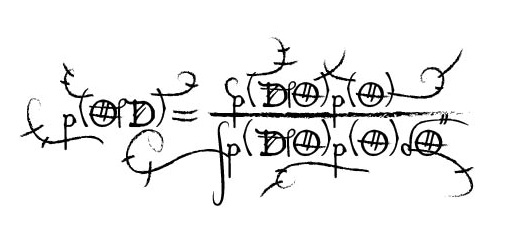
\includegraphics[width=1.5in]{Bayes.jpg}\hfil}\vfil}
%}

{
%\usebackgroundtemplate{\begin{center}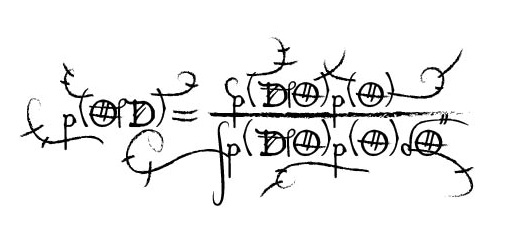
\includegraphics[width=0.4\paperwidth]{Bayes.jpg}\end{center}}
\usebackgroundtemplate{%
  \vbox to \paperheight{\hbox to \paperwidth{\hfil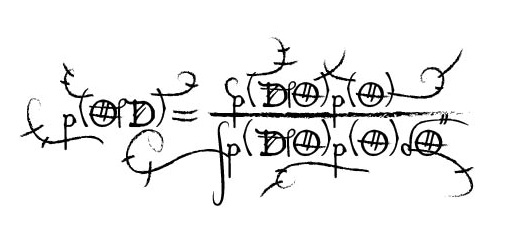
\includegraphics[width=2in]{Bayes.jpg}\hfil}}
}
\begin{frame}
\titlepage
\end{frame}
}
%\frame{\titlepage} 

%\frame{\frametitle{Overview of the talk}\tableofcontents}



\begin{frame}{Lecture overview}

\begin{itemize}
\item Large sample theory
\bigskip
\item Classification
\bigskip
\item Naive Bayes (generative)
\bigskip
\item Logistic regression (discriminative)
\end{itemize}
\end{frame}


\begin{frame}{The likelihood dominates the prior}

%\small{
\vspace{-5mm}
\begin{center}
%\small{
\begin{minipage}{\columnwidth}
\begin{varblock}[0.95\columnwidth]{\color{yellow}A statement I made during the first lecture}
The influence of the prior \textbf{vanishes} as more data is collected. In other words, \textbf{in large samples} \textbf{\color{blue}the likelihood dominates the prior}. Any reasonable prior results in \textbf{essentially the same inferences}.
\end{varblock}

\end{minipage} %}
\end{center}

\begin{itemize}
\bigskip
\item Recall the \textbf{spam data example}: 
\item[] George has gone through his collection of $4601$ e-mails. He classified
$1813$ of them to be spam (and 2788 non-spam).\bigskip{}
\item Four different priors gave the \textbf{same result}.
\end{itemize}

\end{frame}



\begin{frame}{The likelihood dominates the prior, cont.}
%\begin{itemize}
%\item Four different priors give very similar results
%\end{itemize}
\begin{center}
%\includegraphics[scale=0.5,bb = 0 0 200 100, draft, type=eps]{/Users/matvi05/Dropbox/Projects/BayesBook/Figures/SpamDataFull.eps}
\includegraphics[width=1\columnwidth]{SpamDataFull}

\par\end{center}


\end{frame}

\begin{frame}{The likelihood dominates the prior, cont.}
%\begin{itemize}
%\item Four different priors give very similar results
%\end{itemize}
\begin{center}
%\includegraphics[scale=0.5,bb = 0 0 200 100, draft, type=eps]{/Users/matvi05/Dropbox/Projects/BayesBook/Figures/SpamDataFull.eps}
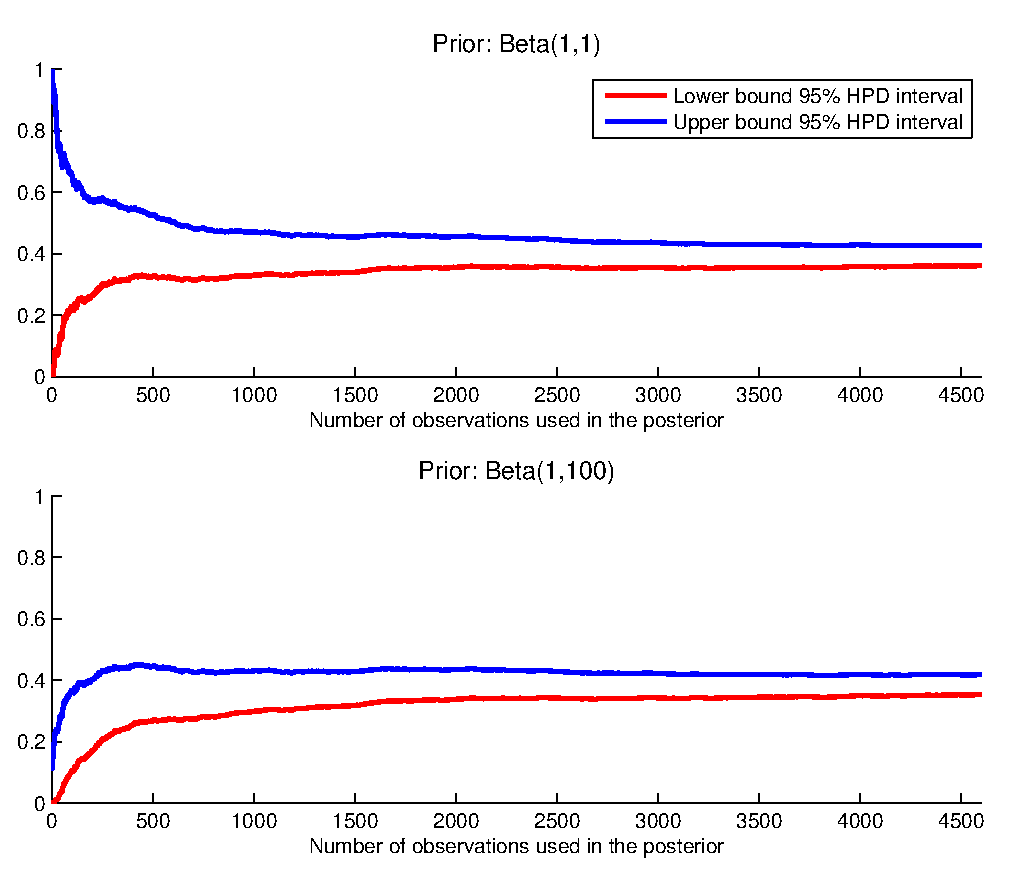
\includegraphics[width=0.8\columnwidth]{spamConvergencePosterior}

\par\end{center}


\end{frame}


\begin{frame}{The behaviour of the posterior as the sample size increases.}
\begin{itemize}
\item \textbf{\color{blue}Recall:} In small samples it was \textbf{\color{red}far from } a normal distribution... 
\end{itemize}

\begin{center}
%\includegraphics[scale=0.5,bb = 0 0 200 100, draft, type=eps]{/Users/matvi05/Dropbox/Projects/BayesBook/Figures/SpamDataFull.eps}
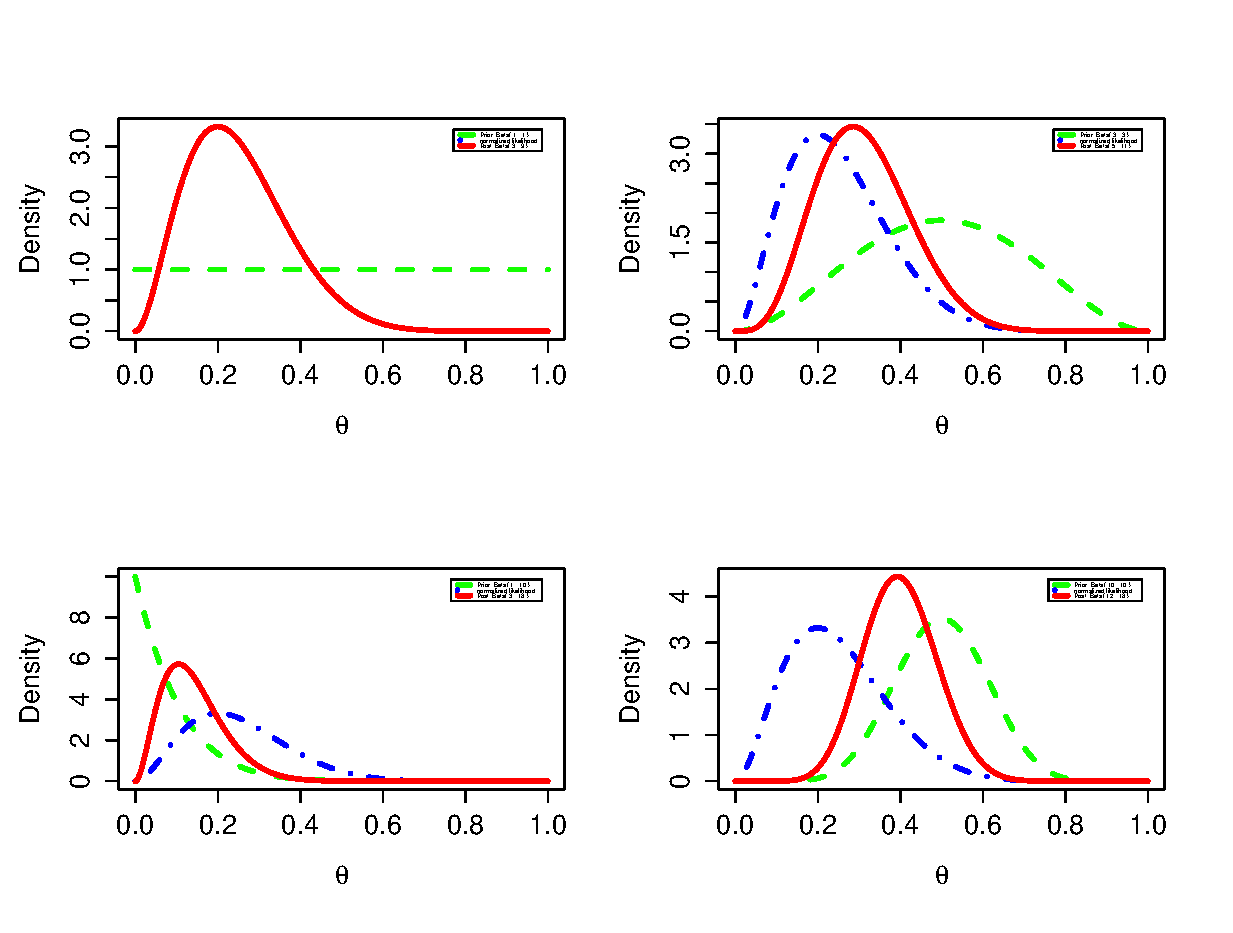
\includegraphics[width=0.9\columnwidth]{SpamDataSmall}

\par\end{center}


\end{frame}


\begin{frame}{The behaviour of the posterior as the sample size increases}
\begin{itemize}
\item ... as \textbf{\color{blue}more data} entered the estimation, normality becomes more reasonable...
\end{itemize}

\begin{center}
%\includegraphics[scale=0.5,bb = 0 0 200 100, draft, type=eps]{/Users/matvi05/Dropbox/Projects/BayesBook/Figures/SpamDataFull.eps}
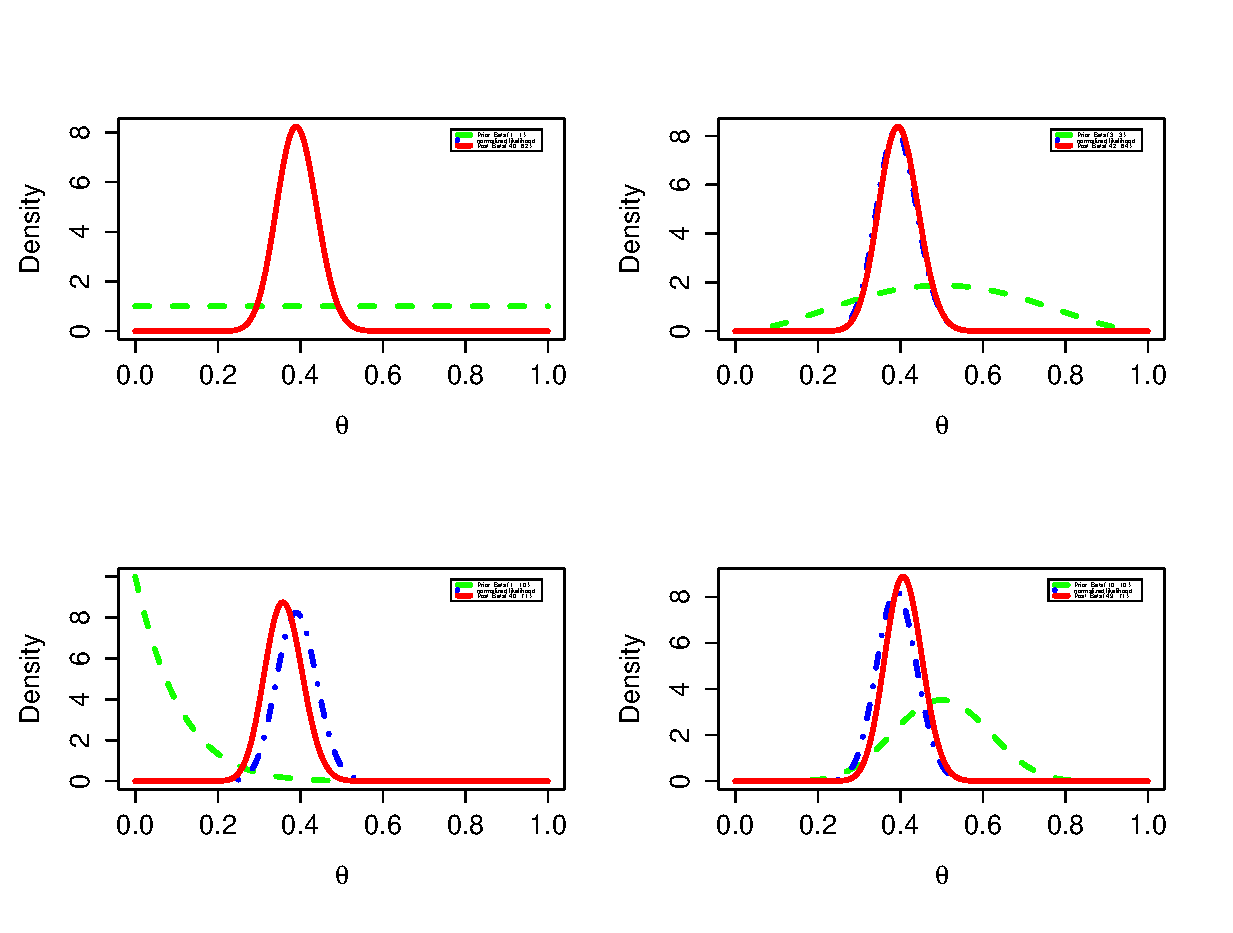
\includegraphics[width=0.9\columnwidth]{SpamDataMedium}

\par\end{center}



\end{frame}



\begin{frame}{The behaviour of the posterior as the sample size increases}
\begin{itemize}
\item ... and with all data (a \textbf{large} sample)... Note that it also \textbf{\color{blue}concentrates}...
\end{itemize}

\begin{center}
%\includegraphics[scale=0.5,bb = 0 0 200 100, draft, type=eps]{/Users/matvi05/Dropbox/Projects/BayesBook/Figures/SpamDataFull.eps}
\includegraphics[width=0.9\columnwidth]{SpamDataFull}

\par\end{center}



\end{frame}



\begin{frame}{Formalizing the statements}

\begin{itemize}
\item We have made \textbf{\color{blue}three observations} as $n$ \textbf{increases}
\begin{enumerate}
\item The likelihood \textbf{dominates the prior}
\item The posterior \textbf{approaches a normal distribution}
\item The posterior \textbf{concentrates around a value}
\end{enumerate}
\item[2.] {\color{blue}Taylor series} expansion of $\log p(\theta | y)$ w.r.t $\theta	\in \mathbb{R}^{p}$ around the {\color{blue}posterior mode} $\theta^{\star}$ 
\small{\begin{align*}
\log p(\theta|y) & = \log p(\theta^\star|y)+\nabla_{\theta} \log p(\theta^\star|y)^{\prime}(\theta-\theta^{\star}) \\ & +\frac{1}{2!}(\theta-\theta^{\star})^{\prime} \nabla\nabla^{\prime}_{\theta}\log p(\theta^\star|y)(\theta-\theta^{\star})+ \dots
\end{align*}
where 
\begin{eqnarray*}
\nabla_{\theta} \log p(\theta^\star|y) &=& \frac{\partial\ln p(\theta|y)}{\partial\theta}\bigg|_{\theta=\theta^{\star}} \in \mathbb{R}^{p} \quad \phantom{11} (\textbf{\color{blue}gradient})\\
\nabla\nabla^{\prime}_{\theta} \log p(\theta^\star|y) &=& \frac{\partial^2\log p(\theta|y)}{\partial\theta\partial\theta^{\prime}}\bigg|_{\theta=\theta^{\star}} \in \mathbb{R}^{p\times p} \quad (\textbf{\color{blue}Hessian})
\end{eqnarray*}}
\end{itemize}

\end{frame}

\begin{frame}{Formalizing statement nbr 2.}

\begin{itemize}
\item Define the \textbf{observed information} $$J_y(\theta^{\star}) = -\nabla\nabla^{\prime}_{\theta} \log p(\theta^\star|y) \quad (\textbf{\color{blue}negative Hessian})$$
\item At the mode \textbf{the gradient} is zero ({\color{red}necessary condition} to be a mode) $$\nabla_{\theta} \log p(\theta^\star|y)=\mathbf{0}$$ 
\item The Taylor series..
\begin{align*}
\log p(\theta|y) & = \log p(\theta^\star|y)-\frac{1}{2!}(\theta-\theta^{\star})^{\prime} J_y(\theta^{\star})(\theta-\theta^{\star})+ \dots
\end{align*}
\item ... can be truncated (in \textbf{\color{blue}large samples})
\begin{align*}
\log p(\theta|y) & \approx \log p(\theta^\star|y)-\frac{1}{2!}(\theta-\theta^{\star})^{\prime} J_y(\theta^{\star})(\theta-\theta^{\star})
\end{align*}
\item ... which is a \textbf{\color{blue}quadratic form} in $\theta$... $p(\theta|y)$ is $\propto$ a normal density!
\end{itemize}

\end{frame}


\begin{frame}{Formalizing statement nbr 2., cont.}

\begin{itemize}
\item Taking exponents
\begin{align*}
p(\theta|y) & \approx \underbrace{p(\theta^\star|y)}_{c} \exp\left(-\frac{1}{2}(\theta-\theta^{\star})^{\prime} J_y(\theta^{\star})(\theta-\theta^{\star})\right)\propto \mathcal{N}_p(\theta^{\star}, J^{-1}_y(\theta^{\star})).
\end{align*}
\bigskip
\item \textbf{\color{blue}Why is this useful?}
%\small{
\item[] We can approximate the posterior of (many) complex (non-conjugate) models by a normal distribution...
%\medskip
\item[] ... but note that we require the {\color{red}posterior mode} and {\color{red}the Hessian} \textbf{evaluated at the mode}...
\item[] ... can easily be obtained with numerical optimization (e.g. \texttt{optim} in \texttt{R}).
%}
\bigskip
\item \textbf{\color{red}But be aware} 
\item[] Posterior might be \textbf{multi-modal}. 
\item[] \textbf{Rate of convergence} depends on $p$. Large $p$ will require \textbf{very large} $n$.

\end{itemize}

\end{frame}


\begin{frame}{Formalizing statement nbr 1.}

\begin{itemize}
\item[1.] \textbf{\color{blue}Recall}: The likelihood dominates the prior. 
\item Assume conditionally iid. observations
$$p(y|\theta) = \prod_{i=1}^n p(y_i | \theta)\quad \text{and} \quad \ell(\theta) = \log p(y|\theta) = \sum_{i=1}^n \log p(y_i | \theta)=\sum_{i=1}^n \ell_i(\theta).$$
\item \textbf{\color{blue}Bayes' theorem} in log scale $\log p(\theta|y) = \log p(y|\theta) + \log p(\theta) + c$
\item Since $$\nabla\nabla^{\prime}_{\theta} \log p(\theta^\star|y) = \nabla\nabla^{\prime}_{\theta} \ell(\theta^{\star}) + \nabla\nabla^{\prime}_{\theta} \log p(\theta^\star)$$
the observed information is
\small{
$$J_y(\theta^{\star}) = \left(-\sum_{i=1}^n J_{y_i}(\theta^{\star})\right) ~ -J(\theta^{\star}),~   J_{y_i} = -\nabla\nabla^{\prime}_{\theta} \ell_i(\theta) \quad  J(\theta^{\star})= -\nabla\nabla^{\prime}_{\theta} \log p(\theta^\star) $$
}
\normalsize
%\normal{
\item[3.] As $n$ increases the curvature is \textbf{dominated} by the information part coming from the likelihood. \textbf{\color{blue}Recall} $$\Sigma_n=J^{-1}_y(\theta^{\star})\quad [\text{The posterior covariance}]$$.
\end{itemize}
\end{frame}


\begin{frame}{Formalizing statement nbr 3.}

\begin{itemize}
\item \textbf{\color{blue}Recall}: The posterior concentrates around a value.
\item \textbf{\color{red}Posterior consistency}: the posterior degenerates to the "\textbf{true value}".
$$\text{"A value" = "the true value"}$$
\item \textbf{But what is the "true value"?}
\begin{itemize}
\item \textit{Mathematical idealization}. \\
 Let $\Theta$ denote the parameter space. The value $\theta_0$ is the "true value" in the sense that the data $$y \sim f(y)=p(y|\theta_0) \quad \text{for some } \theta_0 \in \Theta. $$  
\item \textbf{\color{red}Note}: the data is random ($\theta_0$ is a fixed constant).
\end{itemize}
\item \textbf{Proof}: similar but replacing $J_i(\theta^{\star})$ by the expected information $$I_i(\theta_0) = -E_{y_i}\left(\nabla\nabla^{\prime}_{\theta} \log p(y_i|\theta_0)\right)\quad \text{so that } I(\theta_0)=\sum	_{i=1}^n I_i(\theta_0)$$
is the \textbf{\color{blue}Fisher information}.
\end{itemize}
\end{frame}

\begin{frame}{Example: Normal approximation of a gamma posterior}

\begin{itemize}
\item \textbf{\color{blue}Poisson model}: $\theta\vert y_{1},...,y_{n}\sim \mathrm{Gamma}(\alpha_0+\sum\nolimits _{i=1}^{n}y_{i},\beta_0+n)$
\[
\log p(\theta|y_{1},...,y_{n})\propto(\alpha_0+\sum\nolimits _{i=\mbox{}1}^{n}y_{i}-1)\log(\theta)-\theta(\beta_0+n)
\]

\item First derivative (\textbf{\color{blue}gradient} for $p=1$) of log density
\[
\frac{\partial\log p(\theta|y)}{\partial\theta}=\frac{\alpha_0+\sum\nolimits _{i=\mbox{}1}^{n}y_{i}-1}{\theta}-(\beta_0+n)=0 \implies \theta^{\star}=\frac{\alpha_0+\sum\nolimits _{i=\mbox{}1}^{n}y_{i}-1}{\beta_0+n}
\]
\item Second derivative (\textbf{\color{blue}Hessian} for $p=1$) at mode $\theta^{\star}$ 
\[
\frac{\partial^{2}\log p(\theta|y)}{\partial\theta^{2}}\bigg|_{\theta=\theta^{\star}}=-\frac{\alpha_0+\sum\nolimits _{i=\mbox{}1}^{n}y_{i}-1}{\left(\frac{\alpha_0+\sum\nolimits _{i=\mbox{}1}^{n}y_{i}-1}{\beta_0+n}\right)^{2}}=-\frac{(\beta_0+n)^{2}}{\alpha_0+\sum\nolimits _{i=\mbox{}1}^{n}y_{i}-1}.
\]

\item The \textbf{normal approximation} is
\[
\mathcal{N}\left(\frac{\alpha_0+\sum\nolimits _{i=1}^{n}y_{i}-1}{\beta_0+n},\frac{\alpha_0+\sum\nolimits _{i=1}^{n}y_{i}-1}{(\beta_0+n)^{2}}\right).
\]

\end{itemize}
\end{frame}

\begin{frame}{Example: Normal approximation of a gamma posterior, cont.}


\begin{center}
\includegraphics[scale=0.55]{NormalApprox2Gamma}
\par\end{center}

\end{frame}


\begin{frame}{Normal approximation of posterior}

\begin{itemize}
\item For complex models / high dimensional $\theta$ use standard \textbf{\textcolor{blue}{optimization routines}} (e.g. \texttt{optim} in \texttt{R}). 
\begin{itemize}
\item \textbf{\textcolor{blue}{Input}}: an expression \textbf{proportional to} $\log p(\theta|y)$
and initial values.
\item \textbf{\textcolor{blue}{Output}}: $\log p(\theta^{\star}|y)$, $\theta^{\star}$ and Hessian matrix [$-J_{y}(\theta^{\star})$].\medskip{}

\end{itemize}
\item \textbf{\textcolor{blue}{Re-parametrization}} may improve normal approximation.
{[}Don't forget the \textbf{Jacobian}!{]}

\begin{itemize}
\item If $\theta\geq0$ use $\phi=\log(\theta)$. 
\item If $0\leq\theta\leq1$, use $\phi=\log[\theta/(1-\theta)]$.\medskip{}

\end{itemize}

\item \textbf{\color{blue}Recall change of variables}: Let $p_\theta(\theta)$ be continuous and let $\phi=h(\theta)$ be a one-to-one transform.
$$p_\phi(\phi)=p_\theta(h^{-1}(\phi))|J|, \quad |J|=\text{determinant of } h^{-1}(\phi) \left[1\mathrm{-dim:}~\frac{d}{d\phi}h^{-1}(\phi)\right].$$
\item Even if $p(\theta|y)\approx \mathcal{N}$, $g(\theta)$ may have a \textbf{\color{red}very complex} posterior... 
\item... The \textbf{joy of simulating} to the rescue!
\end{itemize}
\end{frame}


\begin{frame}{Bayesian classification}

\begin{itemize}
\item \textbf{\color{blue}Classification} is like \textbf{regression} but with a {\color{red}discrete label} as output.
\item \textbf{\textcolor{blue}{Examples}}.
\begin{itemize}
\item binary (0-1). Spam/Ham.
\item Multi-class. ($c=1,2,...,C$). $\{iPhone,Android,Windows,Other\}$.
\end{itemize}
\item Let $x=(x_{1},...,x_{p})^{\prime}$ be a vector of $p$ \textbf{\color{blue}covariates/features} (inputs).
\item \textbf{Posterior distribution} over the classes (output) $$\Pr(c=k|x),\quad	k=1,\dots, C \quad [=p(c|x)].$$
\item The \textbf{\textcolor{blue}{Bayesian}} classifies
\[
\underset{c\in\mathcal{C}}{\mathrm{argmax}}\:p(c|x)
\]
\item \textbf{Two approaches}
\begin{enumerate}
\item \textbf{\textcolor{blue}{Discriminative models}} - model $p(c\vert x)$ directly (logistic regression, SVM)\medskip
\item \textbf{\textcolor{blue}{Generative models}} - Use Bayes' theorem $p(c|x)\propto p(x|c)p(c)$
and model \begin{itemize}
\item[(i)] the \textbf{\color{red}class-conditional distribution} $p(x \vert c)$
\item[(ii)] the \textbf{{\color{red}prior}} $p(c)$.
\end{itemize}
% class-conditional distribution $p(\mathbf{x}\vert c)$ and
%prior $p(c)$.
\textbf{Examples:} discriminant analysis, naive Bayes.
\end{enumerate}
\end{itemize}
\end{frame}

\begin{frame}{Generative model: Naive Bayes}

\begin{itemize}
\item By \textbf{\color{blue}Bayes' theorem}
\[
p(c|x)\propto p(x|c)p(c)
\]
\item \textbf{Example:} Let $c=\{\text{\color{red}male}, \text{\color{red}female}\}$ and $x = \{\text{\color{red}weight}, \text{\color{red}length}, \text{\color{red}shoe size}\}$
\item \textbf{Data:} $\{c_i, x_i\}_{i=1}^n$
\item $p(c)$ can be estimated by a conjugate \textbf{\color{blue}Bernoulli-Beta} model with data $c_i, i=1,\dots, n$  (or \textbf{\color{blue}Multinomial-Dirichlet} if $C>2$)
%$c \$
\item \textbf{\color{blue}Non-naive}: $p(x|c)$ can be $\mathcal{N}_{p}(\theta_{c},\Sigma_{c})$ (or more flexibly a \textbf{Finite mixture of normals}, see next module) (\textbf{Note}: $p=3$ in Ex.).
\item \textbf{\textcolor{blue}{Naive Bayes}}: features are \textbf{assumed
independent}\[
p(x|c)=\prod_{j=1}^{p}p(x_{j}|c) \implies p(c|x)\propto\left[\prod_{j=1}^{p}p(x_{j}|c)\right]p(c),
\]
\textbf{\color{blue}Note:} the \textbf{class-conditionals} are modeled separately.
\item \textbf{\color{blue}Classify} using probabilities, e.g. $x = \{\text{52 kg, 160 cm, 36}\}$ \small $$\Pr(\text{\color{red}female} | x) \propto p(x_1=52|\text{\color{red}female})p(x_2=160|\text{\color{red}female})p(x_3=36|\text{\color{red}female})\Pr(\text{{\color{red}female}})$$
\normalsize
\end{itemize}
\end{frame}

\begin{frame}{Generative model: Naive Bayes, cont.}

\begin{itemize}
\item The \textbf{\color{blue}Naive Bayes} is not necessary a realistic model. \bigskip
\item \textbf{Our example}: variables are probably \textbf{\color{red}dependent} (even if gender is known)
\bigskip
\item Why don't \textbf{always} go \textbf{\color{blue}non-Naive}?
\begin{enumerate}
\item Feature vector $x$ might be \textbf{very} high-dimensional.
\item Even with binary features the sample space of $x$ can be \textbf{huge}.
\end{enumerate}
\end{itemize}
\end{frame}


\begin{frame}{Discriminative model: logistic regression}

\begin{itemize}
\item Response is assumed to be \textbf{\textcolor{blue}{binary}} ($y=0$
or $1$).
\item \textbf{\color{blue}Example}: Spam ($y=1$) or Ham ($y=0$). \textbf{Covariates}: $\$$-symbols,
etc.
\item \textbf{\textcolor{blue}{Logistic regression}}
\[
\Pr(y_{i}=1\text{ }|\text{ }x_{i})=\frac{\exp(x_{i}^{\prime}\beta)}{1+\exp(x_{i}^{\prime}\beta)}.
\]

\item \textbf{\color{blue}Likelihood}
\[
p(y|\beta)=\prod\nolimits _{i=1}^{n}\frac{[\exp(x_{i}^{\prime}\beta)]^{y_{i}}}{1+\exp(x_{i}^{\prime}\beta)}.
\]
\textbf{\color{red}Note:} implicitly conditioning on covariates (they are not modeled)
\item \textbf{Our example here}: 
$x_i = \{\text{\color{red}weight}, \text{\color{red}length}, \text{\color{red}shoe size}\}$, for the $i$th obs.
\[
\Pr(y_{i}=\text{\color{red}female}\text{ }|\text{ }x_{i})=\frac{\exp(x_{i}^{\prime}\beta)}{1+\exp(x_{i}^{\prime}\beta)}.
\]
\textbf{\color{red}Note:} \textbf{not} modeling weight/length/shoe size as in the generative model.


\item \textbf{\color{blue}Prior} $\beta\sim N(0,\lambda^{-1}I)$ (simple shrinkage prior). \textbf{\color{blue}Posterior} is \textbf{non-standard}.

\end{itemize}
\end{frame}


\begin{frame}{Discriminative model: logistic regression, cont.}

\begin{itemize}
\item {\color{blue}Markov Chain Monte Carlo} (MCMC) can be used to simulate $p(\beta|y)$.
\bigskip
\item We can alternatively obtain a \textbf{\color{blue}normal approximation} of $p(\beta|y)$.
\bigskip 
\item \textbf{\color{blue}Homework}: Go through \texttt{MainOptimizeSpam.R}. 
\begin{itemize}
\item \textbf{Learn how to master} the function \texttt{optim}
\item \textbf{Learn how to code} an expression of the log posterior (only $\propto$ required)
\item \textbf{Add a step} where you (given the output from \texttt{optim}) simulate from the posterior. \textbf{Hint}:
$$p(\beta|y) \approx \mathcal{N}\left(\theta^{\star}, \Sigma_{\star}\right) \quad \left[\theta^{\star}\text{: mode}, \Sigma_{\star}\text{: -Hess}^{-1}(\theta^{\star}) \right].$$
\end{itemize}
\bigskip 
\item Generalization to \textbf{\color{blue}multi-class} ($c=1,\dots,C$) \textbf{logistic regression}
\[
\Pr(y_{i}=c\text{ }|\text{ }x_{i})=\frac{\exp(x_{i}^{\prime}\beta_{c})}{\sum_{k=1}^{C}\exp(x_{i}^{\prime}\beta_{k})}.
\]

\end{itemize}
\end{frame}





\end{document}

